\documentclass[border=12pt]{standalone}
\usepackage{tikz}
\usepackage{amsmath}
\usetikzlibrary{positioning,arrows.meta,fit,backgrounds,calc}
\begin{document}
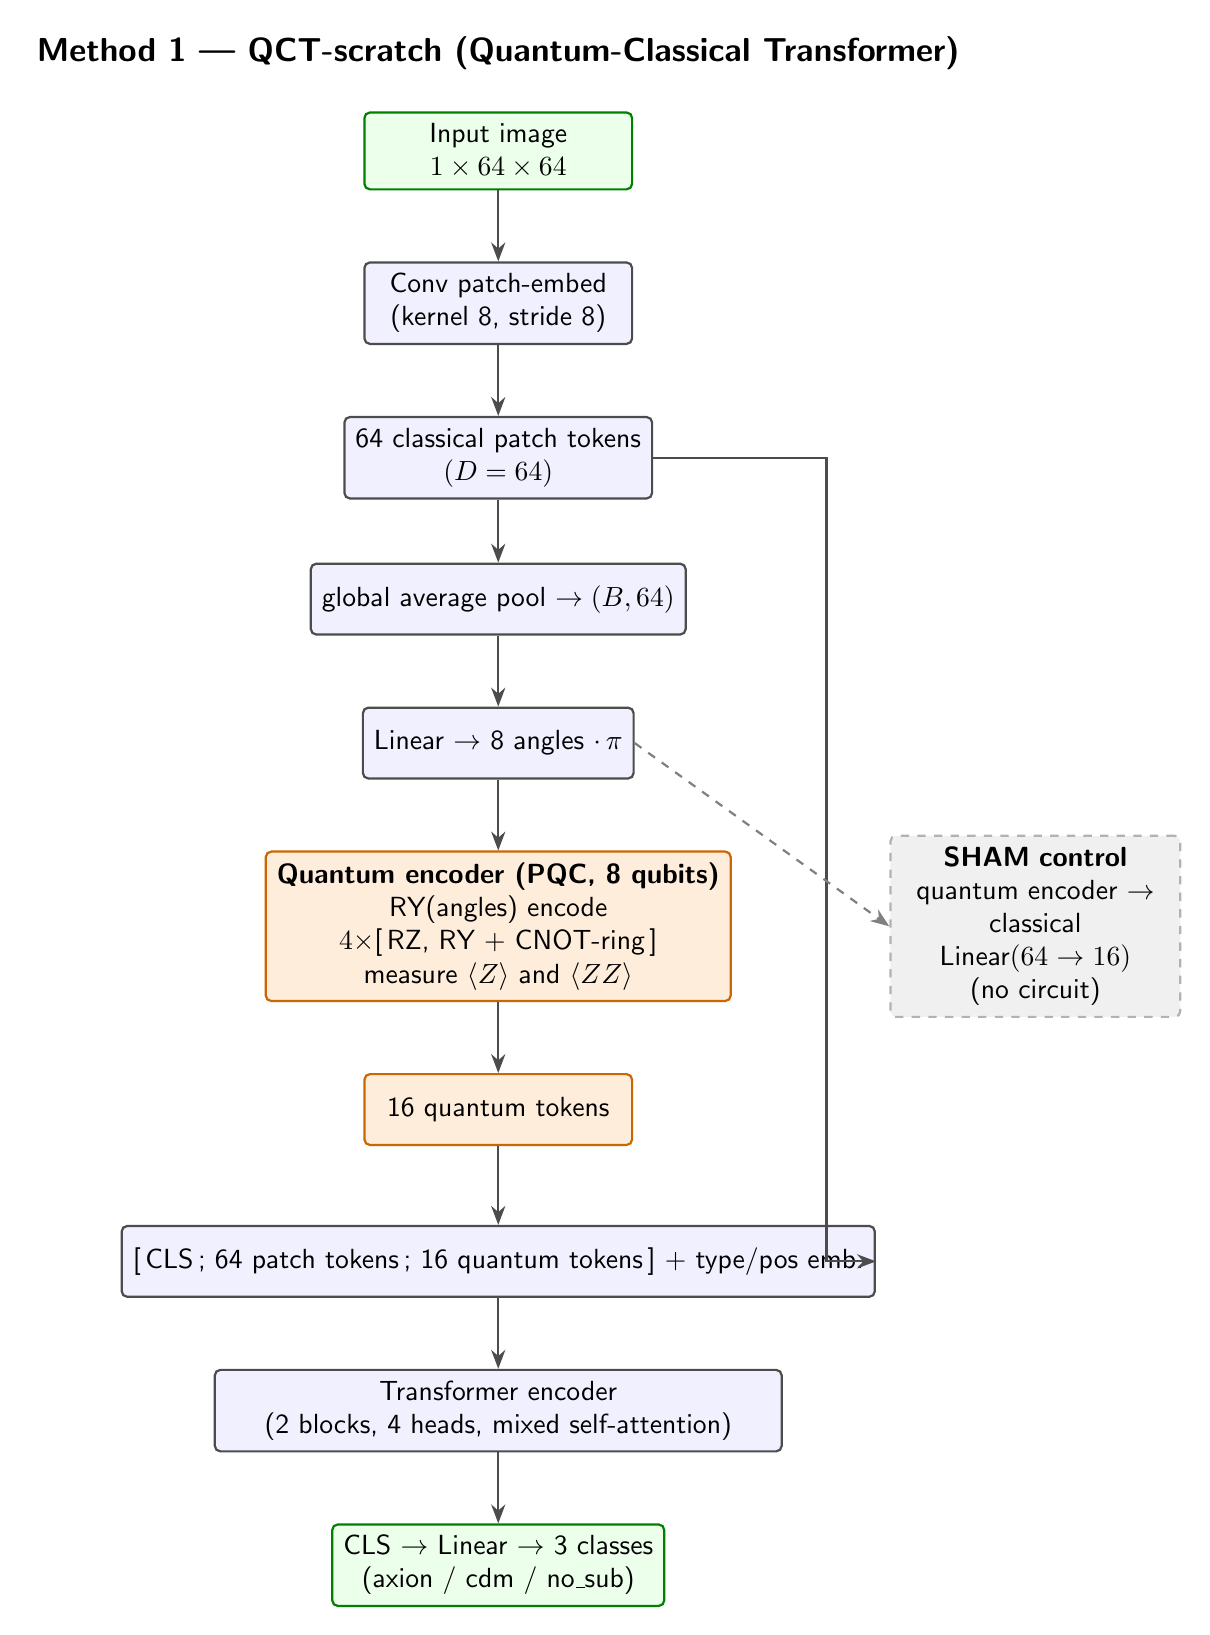
\begin{tikzpicture}[
  font=\sffamily,
  node distance=9mm,
  box/.style={rectangle,rounded corners=2pt,draw=black!70,thick,fill=blue!6,
              minimum height=9mm,minimum width=34mm,align=center,inner sep=4pt},
  qbox/.style={box,fill=orange!14,draw=orange!80!black},
  shbox/.style={box,fill=gray!12,draw=gray!60,dashed},
  io/.style={box,fill=green!8,draw=green!50!black},
  arr/.style={-{Stealth[length=2.4mm]},thick,black!70},
]
\node[io] (img) {Input image\\$1\times64\times64$};
\node[box,below=of img] (patch) {Conv patch-embed\\(kernel 8, stride 8)};
\node[box,below=of patch] (tok) {64 classical patch tokens\\$(D=64)$};
\node[box,below=8mm of tok] (pool) {global average pool $\to (B,64)$};
\node[box,below=of pool] (ang) {Linear $\to$ 8 angles $\cdot\,\pi$};
\node[qbox,below=of ang] (pqc) {\textbf{Quantum encoder (PQC, 8 qubits)}\\
   RY(angles) encode\\$4\times$[\,RZ, RY + CNOT-ring\,]\\measure $\langle Z\rangle$ and $\langle ZZ\rangle$};
\node[qbox,below=of pqc] (qtok) {16 quantum tokens};
\node[box,below=10mm of qtok,minimum width=72mm] (seq)
   {[\,CLS\,;\ 64 patch tokens\,;\ 16 quantum tokens\,] + type/pos emb.};
\node[box,below=of seq,minimum width=72mm] (tr)
   {Transformer encoder\\(2 blocks, 4 heads, mixed self-attention)};
\node[io,below=of tr] (out) {CLS $\to$ Linear $\to$ 3 classes\\(axion / cdm / no\_sub)};

\draw[arr] (img)--(patch);
\draw[arr] (patch)--(tok);
\draw[arr] (tok)--(pool);
\draw[arr] (pool)--(ang);
\draw[arr] (ang)--(pqc);
\draw[arr] (pqc)--(qtok);
% classical token path into the sequence
\draw[arr] (tok.east) -- ($(tok.east)+(2.2,0)$) |- (seq.east);
\draw[arr] (qtok)--(seq);
\draw[arr] (seq)--(tr);
\draw[arr] (tr)--(out);

\node[shbox,right=20mm of pqc,text width=34mm] (sham)
   {\textbf{SHAM control}\\quantum encoder $\to$\\classical Linear$(64\!\to\!16)$\\(no circuit)};
\draw[arr,dashed,gray] (ang.east) -- (sham.west);

\node[font=\sffamily\large\bfseries,above=4mm of img]
   {Method 1 — QCT-scratch (Quantum-Classical Transformer)};
\end{tikzpicture}
\end{document}
